%!TEX root=document.tex

\section{Evaluation}
\label{sec:user_study}

The previous section evaluated \SeeDB and our optimizations in terms of 
performance.
In this section, we assess the value of \SeeDB for real data analysis 
scenarios.
We perform this assessment in two stages. 
First, we perform a study to validate our deviation-based distance metric.
We claim that although simple and limited in its scope, our deviation-based
metric can capture significant information about interesting-ness
of a visualization.
In the second stage, we evaluate the value of \SeeDB vs. a manual chart
construction tool.
We seek to demonstrate that \SeeDB can, in fact, lead users to interesting
visualizations faster than a manual chart exploration tool.

\subsection{Validating Deviation-based Utility}
\label{sec:validating_metric}
In recommendation systems literature, the gold standard for evaluating
a ``recommend good items'' \cite{} system is to obtain ground truth 
about user preferences and examine how well system recommendations line
up with ground truth \cite{}.
We adopt the same evaluation strategy.

\stitle{Obtaining Ground Truth}.
To obtain ground truth, we recuited 5 participants with (3 female, 2
male) all graduate students with prior data analysis experience.
We presented them with the Census dataset (from introduction) and the analytical
task from the introduction \mpv{MAKE SURE.}
Participant were presented with the entire set of aggregate visualizations 
for this dataset and were asked to examine each visualization to identify 
visualizations that were interesting {\it in the context of the task}.
Participants were also asked to indicate why they chose a visualization
as interesting.
There was no upper limit on the number of visualizations a participant could
choose.
We capped the study at 10 minutes.

\begin{figure}[t]
	\centering
	\begin{subfigure}{0.45\linewidth}
		{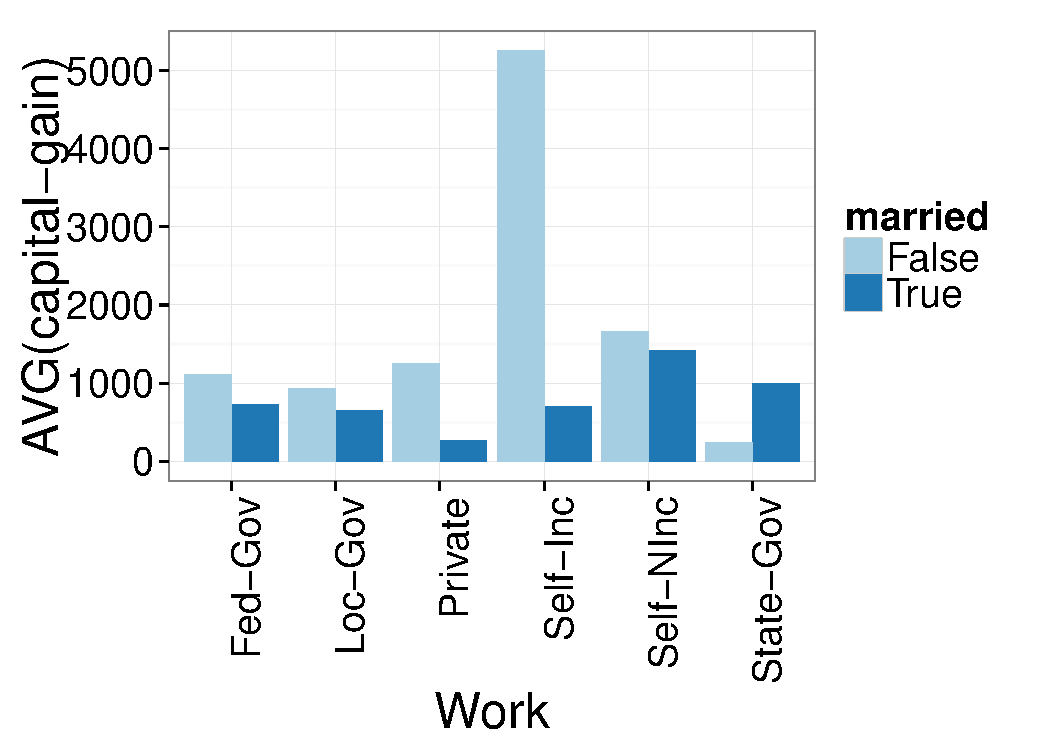
\includegraphics[width=4cm, trim=0 0 3cm 0, clip=true] {Images/HUHI_work_avg_cap_gain.pdf}}
		\caption{Popular Visualization}
		\label{fig:popular}  
	\end{subfigure}
	\begin{subfigure}{0.54\linewidth}
		{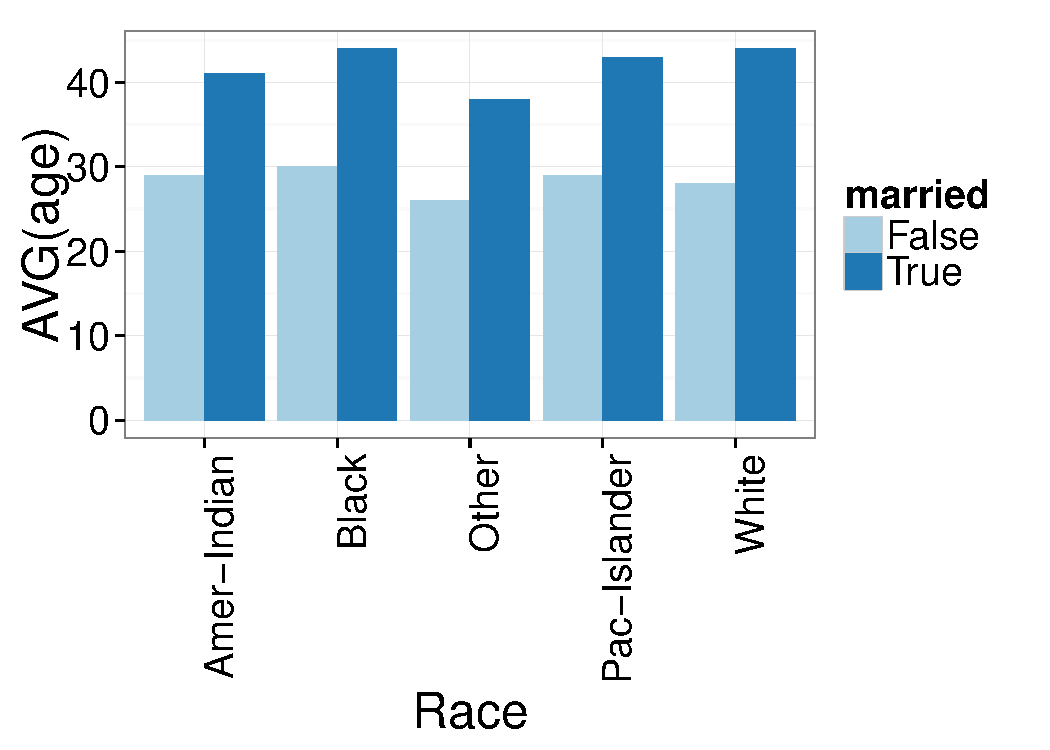
\includegraphics[width=4.5cm] {Images/LULI_race_avg_age.pdf}}
		\caption{Unpopular visualization}
		\label{fig:not_popular}
	\end{subfigure}
	\vspace{-10pt}
	\caption{Baseline performance and Effect of Combining Aggregates }
	\vspace{-10pt}
	\label{fig:gt_examples}
\end{figure} 

Each participant identified between 5 - 10 visualizations as being interesting
in the context of the task.
Figure \ref{ig:intro} in Section \ref{sec:introduction} showed an example of one of the most interesting
visualizations found by our participants () as well as one of the least interesting
(). \mpv{maybe review explanation}
Figure \ref{fig:gt_examples} shows two other examples of visualizations for this
dataset: Figure \ref{fig:popular} 
shows a visualization that was chosen as interesting by 4 of 5 participants.
According to the participants this visualization was relevant because ``\ldots it
showed a big difference in earning for self-inc'' and indicated a trend to 
be examined further.
Figure \ref{fig:not_popular} in contrast shows a visualization that participants
did not select as relevant the distributions showed little difference. 
Figure \ref{} shows a visualization that in fact has high deviation but was not 
found to be relevant. \mpv{should this go here?}
The reason participants did not select the visualization was either because ``\ldots
did not really understand it'' or ``\ldots did not think it was relevant.''
These charts together show that in addition to deviation, participants had other
heuristics for interestingness.

In all, participants selected 23 unique visualizations as being interesting.
To obtain a consensus on ground truth, use used a simple voting system.
Any visualization that was chosen by majority of participants (3 or more)
was considered to the interesting; the rest were not.

\stitle{Efficacy of Deviation-based Metric}.
Once we obtained ground truth, we evaluated whether \SeeDB could recover
the interesting visualizations.
We ran \SeeDB over the same dataset and for the same analytical task.
Figure \ref{fig:gt_dist} shows a heatmap of the number of times each
visualization in the census dataset was selected as being interesting 
({\em yellow} = popular, {\em blue} = not popular).
First, notice that participants had a high level of agreement on the 
visualizations they found interesting.
Of the 23 unique visualizations, majority of participants agreed on 
6 visualizations as being interesting; this suggests that while
there are individual preferences, we can distill general preferences
for visualizations.
next, notice that the utilities in \ref{fig:gt_dist} are sorted in descending order 
from top to bottom.
As we can see from the heatmap, the most {\em popular} visualizations are
the ones with high utility.
We evaluated this trend computationally via an ROC (``receiver operating curve'')
analysis \cite{}.
To construct the ROC curve, we varied the number of visualizations recommended by 
\SeeDB ($k$) and for each $k$ calculated the 
number of true positives (ground truth visualizations recommended by \SeeDB),
false positives (non-ground truth visualizations recommended by \SeeDB), 
true negatives(non-ground truth visualizations not recommended by \SeeDB) and 
false negatives (ground truth visualizations not recommended by \SeeDB).
Figure \ref{fig:roc} shows the ROC curve for \SeeDB and absolute baseline (AUROC = 0.5).
AUROC for \SeeDB is 0.903. 
In general, AUROC values above 0.8 are indicative of high quality recommendations\cite{};
AUROC of 0.9 indicates that \SeeDB (and our deviation metric) performs extremely well in 
recommending visualizations for this task.
We acknowledge however that the ROC (and AUROC)
would vary with difference datasets and anlytical tasks. 
\mpv{IDEALLY GET DATA FOR OTHER DATASETS OR OTHER TASKS ON THE SAME DATASET}

Thus we find that our deviation-based metric does, in fact, identify visualizations that
users find interesting for an analytical task.
In the next section, we examine the effect of providing recommendations during visual 
analysis.

\begin{figure}[t]
	\centering
	\begin{subfigure}{0.3\linewidth}
		{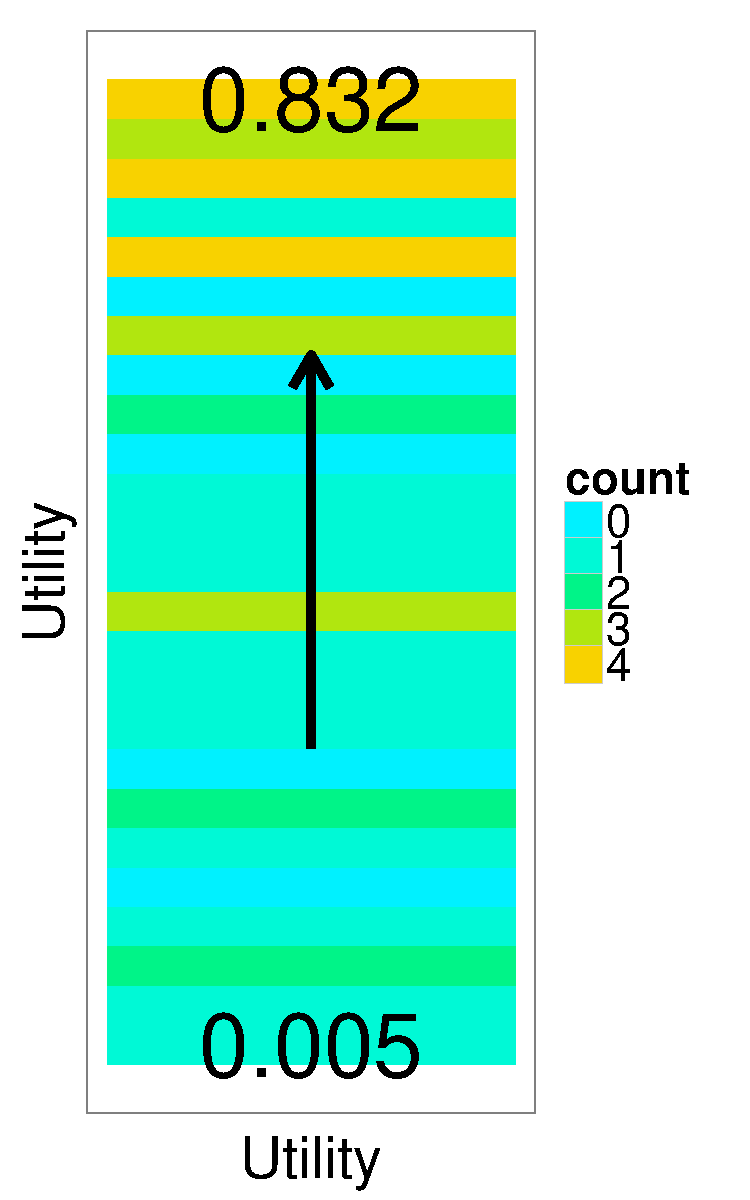
\includegraphics[trim={0 1.3cm 0 0}, clip, width=3cm]{Images/census_gt_distribution.pdf}}
		\caption{Distribution ground truth utilities}
		\label{fig:gt_dist}
	\end{subfigure}
	\begin{subfigure}{0.68\linewidth}
		\centering 
		{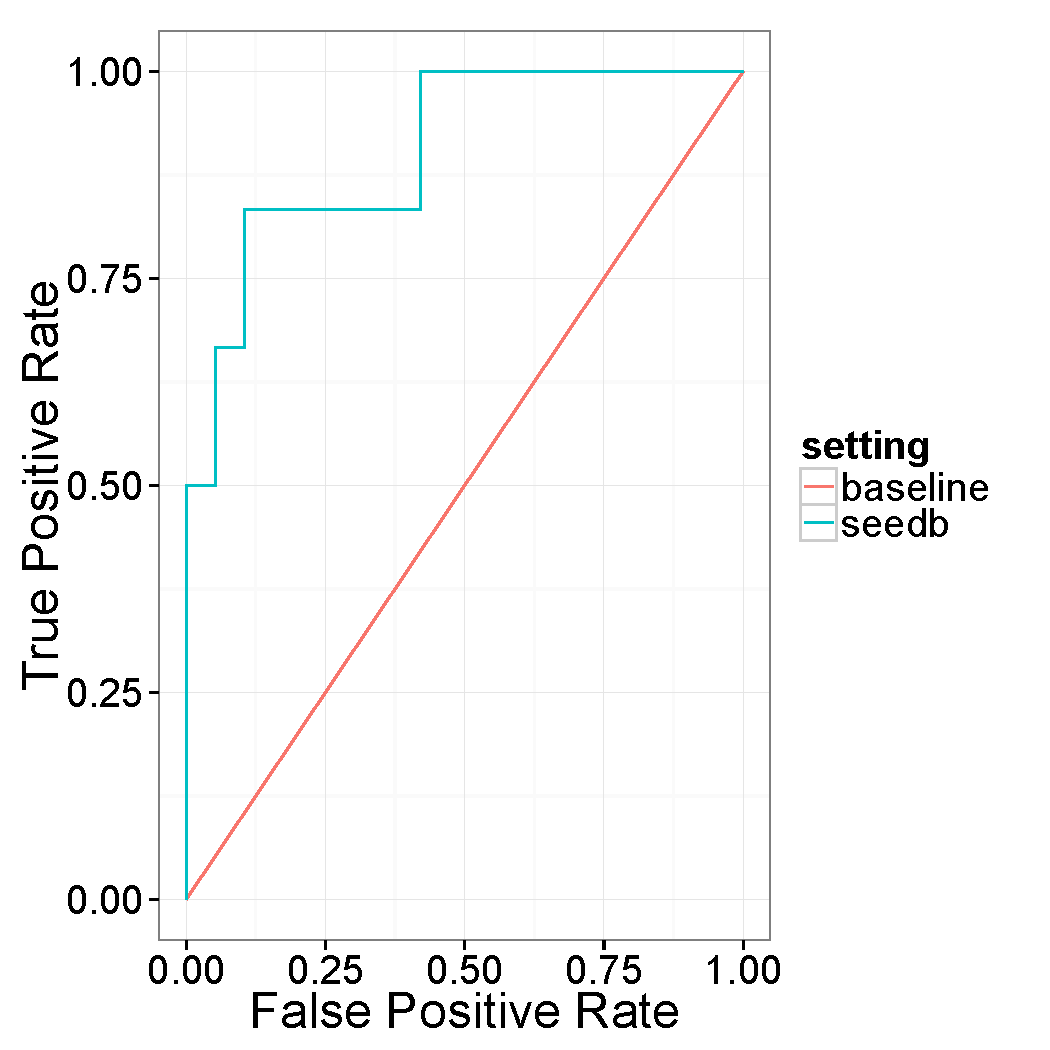
\includegraphics[width=5cm] {Images/seedb_roc.pdf}} 
		\caption{ROC of SeeDB (AUROC = 0.903)}
		\label{fig:roc}
	\end{subfigure}
	\vspace{-10pt}
	\caption{Performance of Deviation metric for Census data}
	\vspace{-10pt}
	\label{fig:census_gt}
\end{figure}

\mpv{user preference?}
\mpv{Something about the new metric}.

\subsection{\SeeDB vs. Manual Chart Construction Tool}
\label{sec:seedb_vs_manual}

To assess the efficacy of \SeeDB in enabling faster visual analysis,
we conducted a user study where participants performed visual analysis
using both \SeeDB and a manual chart construction tool.
We hypothesized that: (i) When using \SeeDB, participants would find 
interesting visualizations {\em faster} than when using manual chart
construction, (ii) Participants would find more interesting visualizations
when using \SeeDB vs. when using manual chart construction, (iii) 
Participants would prefer using a tool with recommendations vs. a manual
construction tool.

\stitle{Participants}. We recruited 16 participants (5 female, 11
 male) all graduate students with prior data analysis experience.
 All subjects had previous experience with visualization tools (e.g.
 R, ggplot, Excel).
 None of the participants had previously worked with any of the study datasets.
 The study lasted \~an hour and participants were compensated with a \$15
 gift card.

 \stitle{Datasets}. We used two datasets during our study:
 (1) {\em Housing} - Dataset of housing prices in
 the Boston area comprising crime rate, racial diversity, housing prices and
 income indicators; 
 (2) {\em Movies} - Dataset about movies containing information about gross
 sales, genres, and ratings;
 These two datasets were chosen because they were easy to understand and 
 their topics that would be familiar to participants. 
 In addition, the datasets were comparable in terms of number of rows and 
 potential visualizations.

\stitle{Study Protocol}.
Our user study used a 2 (visualization tool) X 2 (dataset) 
within-subjects design.
The tools used were \SeeDB and {\em MANUAL}-{\em only} version of \SeeDB.
MANUAL was the same as \SeeDB except that the recommendations bar was 
removed (Figure \ref{}).
Using the same underlying tool in both conditions allowed us to control for
tool-related factors such as functionality and user interface.
We used a within-subjects design to compensate for difference in data analysis
expertise within subjects, and used counterbalancing to remove any effects 
related to order and the test dataset.

Our study began with a short tutorial on the two tools used in the study.
The tutorial used a dataset different from the study datasets and acquainted
the user with the functionality of both tools.
Following the tutorial, participants were asked to perform two visual analysis 
tasks, one with each tool (condition).
In each condition, we introduced participants to the test dataset
and described the analytical prompt using written instructions.
Each analytical task asked participants to use the specific tool to find 
visualizations supporting or disproving a specific hypothesis.
Participants were asked to use the bookmark button (XXX in Figure \ref{}) to 
flag any visualizations they deemed relevant for the particular task.
Participants were also encouraged to think aloud and explain their thought process
while performing the task.
Since the analytical tasks were open-ended, we capped each task at 8 minutes.
After each task, participants filled out a short survey about their experience
using the particular tool.
Most questions were answered on a 5-point Likert scale.
All studies were conducted in a lab setting using Google Chrome on a 15-inch 
Macbook Pro.

\stitle{Methods and Metrics}.
Over the couse of each study session, we collected data by three means: interaction logs 
from each tool, study staff notes, and responses to surveys.
Since users were asked to bookmark visualizations they found to be relevant to the task,
bookmarking behavior, recovered from tool interaction logs, provides the richest source
of information about the analytical process.
Specifically, we study a number of metrics including: (i) number of bookmarks ($num\_bookmarks$), 
(ii) total number of visualizations viewed ($total\_viz$), 
(iii) bookmarking rate ($bookmark\_rate$) defined as $num\_bookmarks$/$total\_viz$, and 
(iv) the time to bookmark ($bookmark\_time$).
\SeeDB and MANUAL support construction of two kinds of charts: aggregate visualizations and 
scatterplots (to replicate real visual analysis).
Since \SeeDB can only recommend aggregate visualizations, we also examine the corresponding
metrics for aggregate visualization only.
We evaluate statistical signifance of our results using paired t-tests and ANOVAs.

% We hypothesize that if a visualization is high-quality, it is more likely to be bookmarked.
% This implies that high-quality recommendations can lead to a larger number of bookmarks and
% an increase in the bookmarking rate.

\stitle{Results}.
Over the course of our study, participants built over 250 visualizations and bookmarked 70
visualizations.
The overall bookmark rate was 0.26.
We next describe our key findings and observations.

\stitle{1. \SeeDB enables fast visual analysis}.
Table \ref{tab:bookmarks} shows an overview of the bookmarking behavior divided by tool.
We find that, in general, participants bookmarked slightly more visualizations with \SeeDB than 
with MANUAL.
On the other hand, we find that participants interacted with fewer visualizations in \SeeDB than
in MANUAL.
As a consequence of these two opposing forces, we find that participants using \SeeDB view fewer
visualizations but bookmark more, i.e., the visualizations they interact with are high quality.
In fact, the $bookmark\_rate$ for \SeeDB is 1.5X higher than that for MANUAL.
We also find that, on average, the $bookmark\_time$ for \SeeDB (92.91 $\pm$ 49.26) is twelve seconds 
shorter than that for MANUAL (105.02 $\pm$ 58.24). 
While these differences are not statistically significant, they point towards a trend: {\it \SeeDB
enables participants to arrive at interesting visualizations faster than MANUAL}.

\begin{table}[htb]
  \centering \scriptsize
  \begin{tabular}{|c|c|c|c|c|} \hline
   & num\_bookmarks & total\_viz & bookmark\_rate \\ \hline
  MANUAL & 3.3 $\pm$ 1.42 & 14.1 $\pm$ 5.4 & 0.24 $\pm$ 0.09 \\ \hline
  \SeeDB & 3.5 $\pm$ 1.35 & 12.1 $\pm$ 4.7 & 0.36 $\pm$ 0.22 \\ \hline
  \end{tabular}
  \vspace{-10pt}
  \caption{All Visualizations: Bookmarking behavior Overview}
  \label{tab:bookmarks} 
  \vspace{-10pt}
\end{table}

Recall that \SeeDB (currently) only supports recommendations for aggregate visualizations.
Therefore views of all visualizations do not necessarily capture the behavior with respect to
aggregate visualizations.
When we examine the same metrics with respect to aggregate visualizations, we find a clear
signal.
The rate of bookmarking aggregate ($agg\_bookmark\_rate$) visualizations in \SeeDB (0.42) is 3X that
in MANUAL (0.14).
The 3X increase is larger than that seen in all visualizations (1.5X) and is statistically significant 
within subjects as well as across subjects ({\em Paired t-test, t = -2.5599, df = 8, p-value = 0.03365}).
We note that there is significant difference also between the number of aggregate bookmarks in the
two conditions.
However, the absolute number of aggregate visualizations and therefore aggregate bookmarks is closely
tied to the relative proportion of scatterplots and aggregate visualizations.
As a result, the absolute numbers can be biased and we ignore them in spite of their statistical
significance.
Finally, we note that a 2-way ANOVA also concurs that the tool has a significant impact on aggregate 
bookmark rate ({\em df = 1, sum sq = 0.3681, mean sq = 0.3681, F value = 10.034, p = 0.00685}). 
We find that choice of dataset does not affect bookmark rate, and there are no interaction or order effects.

User survey data also supports the claim that \SeeDB enables fast analysis.
87\% of participants indicated that \SeeDB recommendations sped up their visual analysis.

\stitle{2. \SeeDB found interesting and unexpected visualizations}.
One of the goals of \SeeDB is to find interesting visualizations that the user may not generate, i.e.,
we want to surface unexpected visualizations.
We find evidence for this in the study.
Figure \ref{} shows an example of visualizations that were not generated by participants using MANUAL
but was in fact recommended by \SeeDB and bookmarked as being interesting.
78\% of participants also indicated that \SeeDB recommended visualizations they might not explored, e.g.
``\ldots interesting aspects of data to compare. I don't think I would have checked those by myself.''.


\stitle{3. \SeeDB provides starting point for analyses}. 
To our knowledge, \SeeDB is the first tool to provide recommendations for supporting visual
analysis.
As a result, we were interested in how recommendations could fit into the analytical workflow.
While a participant's exact workflow was unique, we repeatedly found the pattern {\em recommendation 
$\rightarrow$ manual\_modify $rightarrow$ manual\_modify $rightarrow$ \ldots bookmark}.
Specifically, participants would often start from one of the recommendations and explore other
visualizations that were variations of it (e.g. different aggregation or measure attribute) 
until they found an interesting visualization.
\mpv{can I put any data here?}
Thus, even if recommendations weren't bookmarked directly, their variations were often bookmarked.
This pattern was highlighted in user comments as well. 
8 users highlighted the use of \SeeDB in {\em seeding} their analysis: e.g.,
``\ldots would be incredibly useful in the initial analysis of the data'', 
``Exploratory analysis \ldots'',
``\ldots great tool for proposing a set of initial queries for a dataset'',
``\ldots quickly deciding what correlations are relevant and gives a quick peek''.
On the other hand, we found participants are much less satisfied with recommendations when they 
are unable to interact with or modify them.
These observations reinforce the design choice of \SeeDB as a complement to a traditional
visualization system; the mixed-initiative nature of the system is essential for the system to be
userful in analysis.

\stitle{4. All participants preferred \SeeDB to MANUAL}. 
The most important result of our survey was that 100\% of all users preferred \SeeDB to MANUAL for
visual analysis, i.e., all users preferred to have recommendations while carrying out visual analysis.
As discussed previously, 78\% of participants found the recommendations helpful and thought that they
showed interesting trends.
An interesting observation from two participants was that they did not want to rely too heavily
on the recommendations; one participant noted {\em ``The only potential downside may be that it made 
me lazy so I didn't bother thinking as much about what I really could study or be interested in''}.
This observation suggests that there is a high bar on quality for recommendations, and an interesting
line of future work could be to explore means to build confidence in recommendations.

% 86\% of participants indicated that the recommendations sped up their analysis.


% When asked to rate the recommendations provided by \SeeDB, 78\% participants indicated that the
% recommendations were either ``Helpful'' or ``Very Helpful''. 
% We also found that 90\% of participants found the comparative visualizations shown by \SeeDB 
% helpful in their analysis.
% 66\% of participants indicated that the recommendations needed improvement, in particular,
% participants were interested in seeing different types of charts (e.g. geographical, time series)
% and obtaining measures of statistical significance.

% \stitle{Qualitative Feedback}. In their qualitative feedback, participants highlighted the importance of 
% a tool like \SeeDB at the initial stages of analysis. 
% One partitipant said, {\em ``It's a great tool for proposing a set of initial queries for a dataset I have never seen. 
% And from these visualizationns, I can figure out which related patterns to dig into more.''}
% Others thought that the strength of the tool was in quickly finding relevant trends, {\em ``It's a good tool that helps 
% in quickly deciding what correlations are relevant and gives a quick peek''}. 
% Overall, participants indicated that \SeeDB was particularly suited for exploratory analysis of new datasets, 
% {\em ``I thought SeeDB was very helpful in helping me get more familiar with a new dataset quickly.''}.



